\documentclass[12pt,a4paper]{article}


% -------------------------------------------------------------------------
% import common LaTeX settings
% -------------------------------------------------------------------------

\usepackage{import}

\subimport{../}{CommonLaTeXSettings}


% -------------------------------------------------------------------------
\begin{document}
% -------------------------------------------------------------------------

%\noindent

\title{
User's guide to \xmlToLy\ \\[5pt]
}

\author{
Jacques Menu 
}

\date {\normalsize \today\ version}
%\date {}

\maketitle
\thispagestyle{fancy} % right after \maketitle to apply it to the first page too

\abstract {
This document presents the design principles behind \xmlToLy, as well as the way to use it. It is part of the \lib\ documentation, to be found at \url{https://github.com/grame-cncm/libmusicxml/tree/lilypond/doc}.

All the examples mentioned can be downloaded from \url{https://github.com/grame-cncm/libmusicxml/tree/lilypond/files/samples/musicxml}. They are grouped by subject in subdirectories, such as \mxmlfile{basic/HelloWorld.xml}.
}

% -------------------------------------------------------------------------
% -------------------------------------------------------------------------
\section{Acknowledgements}
% -------------------------------------------------------------------------
% -------------------------------------------------------------------------

Many thanks to Dominique Fober, the designer and maintainer of the \lib\ library. This author would not have attempted to work on a \mxml\ to \lily\ translator without it already available.

In particular, the conversion of \mxml\ data to a tree is extremely well done directly from the \mxml\ DTD, and that was a necessary step to produce \lily\ code. Dominique also provided a nice way to browse this tree with a two-phase visitor designe pattern, which this author used extensively in his own code. The interested reader can find information about that in \docpdf{presentation}{libmusicxml2.pdf}.

\xmlToLy\ and some of the specific examples presented in this document are this author's contribution to \lib.


% -------------------------------------------------------------------------
% -------------------------------------------------------------------------
\section{Overview of \xmlToLy\ }
% -------------------------------------------------------------------------
% -------------------------------------------------------------------------

The initial name of \xmlToLy, when it started as a clone of \xmlToGuido, was {\tt xml2lilypond}. Both Dominique Fober and Werner Lemberg, an early tester, found it too long, and they chose \xmlToLy\ among other names this author proposed to them.

% -------------------------------------------------------------------------
\subsection{Why \xmlToLy?}
% -------------------------------------------------------------------------

\lily\ comes with \mxmlToLy, a translator of \mxml\ files to \lily\ syntax, which has some limitations. Also, being written in Python, it is not in the main stream of the \lily\ development and maintainance group. The latter has much to do with C++ and Scheme code already.

After looking at the \mxmlToLy\ source code, and not being a Python developper, this author decided to go for a new translator written in C++.

The design goals for \xmlToLy\ were:
\begin{itemize}
\item to perform at least as well as \mxmlToLy;
\item to provide as many options as needed to adapt the \lcg\ to the user's needs.
\end{itemize}

Speed was not an explicit goal, but as it turns out, \xmlToLy\ is not bad in this respect.

% -------------------------------------------------------------------------
\subsection{What \xmlToLy\ does}
% -------------------------------------------------------------------------

The architecture of \lib, which can also be seen at \docpdf{libmusicxmlArchitecture}{libmusicxmlArchitecture.pdf}, is presented in figure \ref{libmusicxmlArchitecture}.
It shows the place of \xmlToLy\ in the whole.

\begin{figure}
\caption{\lib\ architecture}\mylabel{libmusicxmlArchitecture}
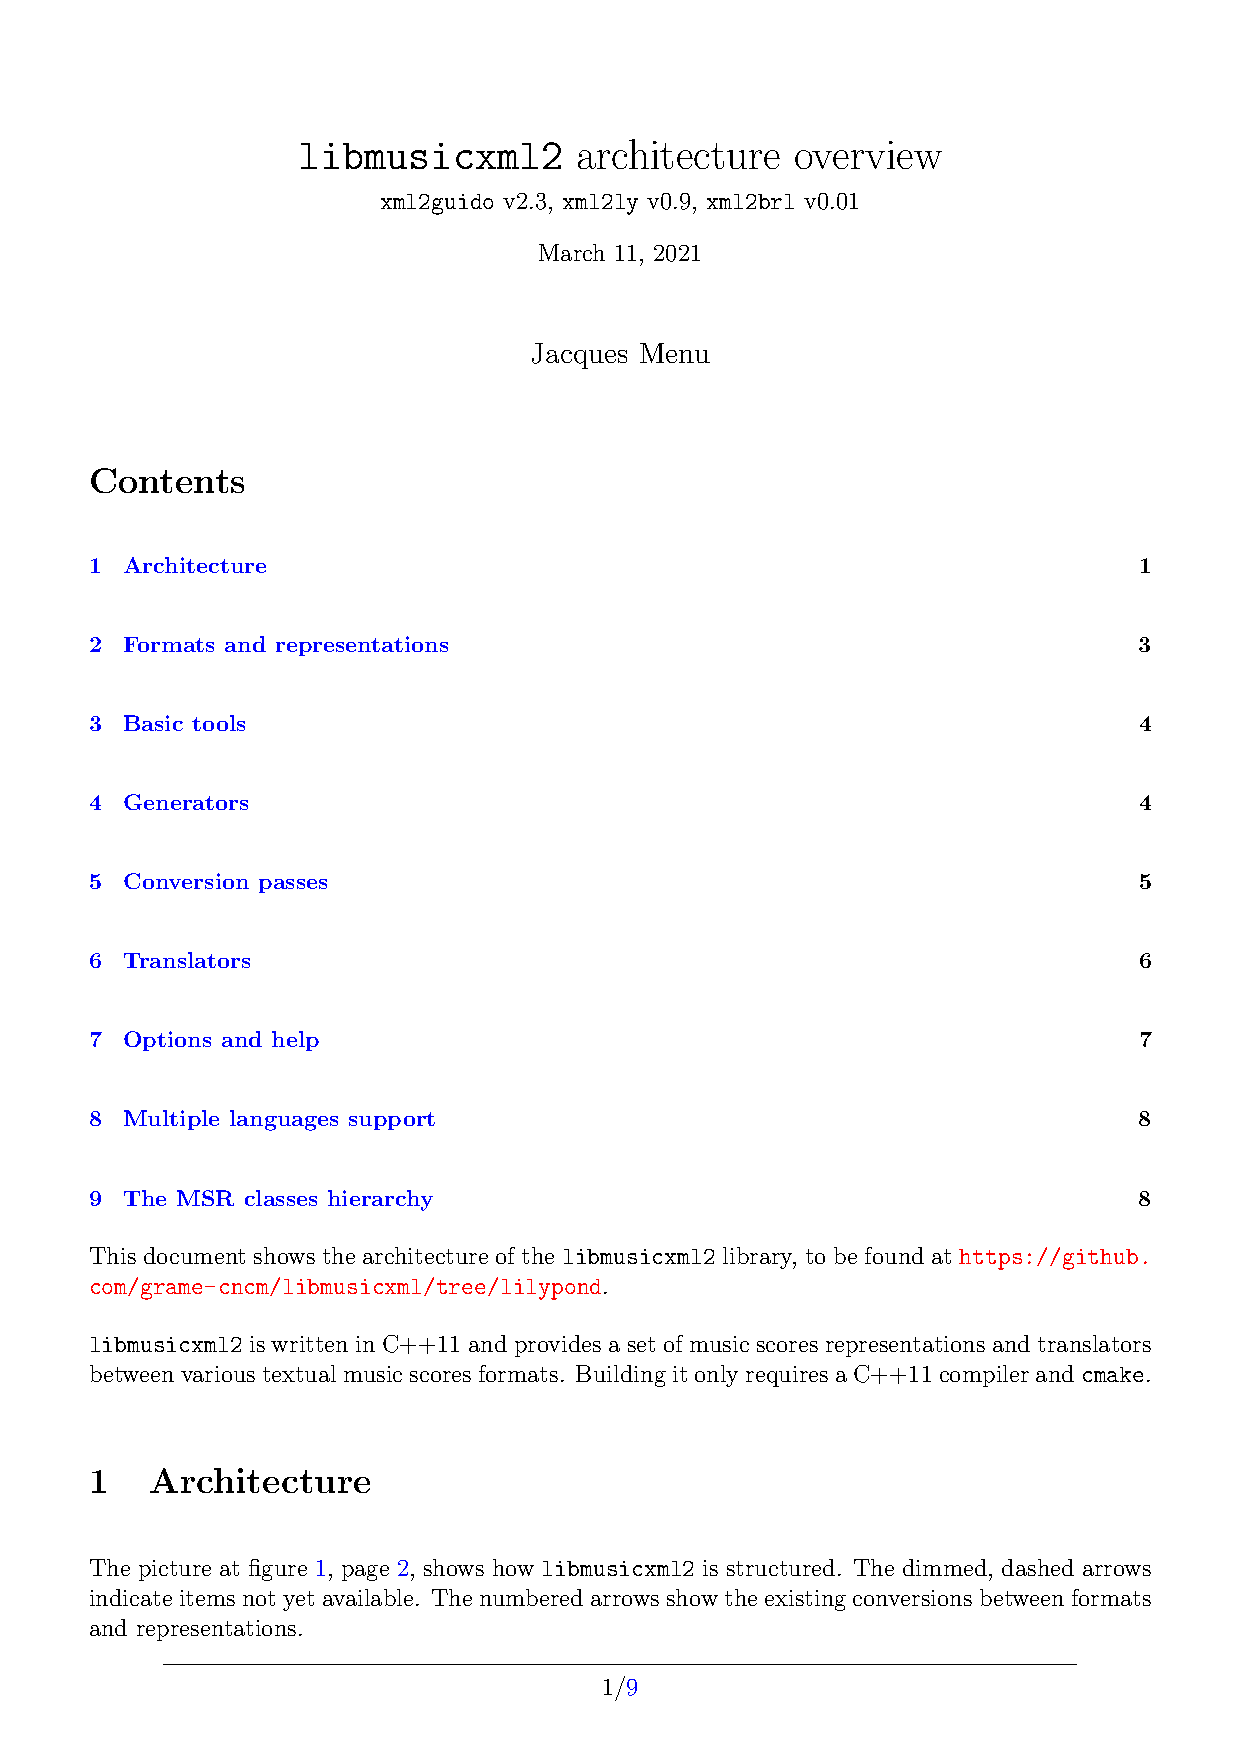
\includegraphics[scale=0.8]{../libmusicxmlArchitecture/libmusicxmlArchitecture.pdf}
\end{figure}

The '{\tt -about}' option to \xmlToLy\ details that somewhat:
\begin{lstlisting}[language=XML]
menu@macbookprojm > xml2ly -about

What xml2ly does:

    This multi-pass translator basically performs 5 passes:
        Pass 1:  reads the contents of MusicXMLFile or stdin ('-')
                 and converts it to a MusicXML tree;
        Pass 2a: converts that MusicXML tree into to
                 a Music Score Representation (MSR) skeleton;
        Pass 2b: converts that tree and the skeleton into a
                 Music Score Representation (MSR);
        Pass 3:  converts the MSR into a
                 LilyPond Score Representation (LPSR);
        Pass 4:  converts the LPSR to LilyPond source code
                 and writes it to standard output.

    Other passes are performed according to the options, such as
    printing views of the internal data or printing a summary of the score.

    The activity log and warning/error messages go to standard error.
\end{lstlisting}


% -------------------------------------------------------------------------
% -------------------------------------------------------------------------
\section{Options and help}
% -------------------------------------------------------------------------
% -------------------------------------------------------------------------

\xmlToLy\ is equipped with a full-fledged set of options with the corresponding help. Since there are many options and the translation work is done in successive passes, the help is organized in a hierarchy of groups, each containing sub-groups of individual options called '{\it atoms}'.

% -------------------------------------------------------------------------
\subsection{Basic principles}
% -------------------------------------------------------------------------

Options are introduced on the command line either by '{\tt -}' or '{\tt --}', which can be used at will. There no difference between the two.

Each option has a short name and an optional long name. The latter is not needed if the short name is sufficiently explicit and not too long, such as '{\tt -jianpu}', '{\tt -cubase}', '{\tt -ambitus}' or '{\tt -custos}'.

Some options have their usual meaning in open-source software, such as '{\tt -h}' (help), '{\tt -a}' (about), and '{\tt -o}' (output file name).

Some options name, short or long, share a common prefix, which allows them to be contracted, as in '{\tt -h=msr,lily}', which is equivalent to '{\tt -msr, -lily}', and '{\tt -trace=voices,notes}', equivalent to '{\tt -trace-voices, -trace-notes}'.

There are single-character options, which can be clustered: '{\tt -vac}' is equivalent to: '{\tt -v, -a, -c'}.

% -------------------------------------------------------------------------
\subsection{Introspection}
% -------------------------------------------------------------------------

One can obtain help on any specific group, sub-group or atom, such as:
\begin{lstlisting}[language=XML]
menu@macbookprojm > xml2ly -option-name-help ambitus         

--- Help for option 'ambitus' in subgroup "Engravers" of group "LilyPond" ---

LilyPond (-hlily, -help-lilypond):
  These lilypond control which LilyPond code is generated.

--------------------------
  Engravers (-hlpe, -help-lilypond-engravers):
  
    -ambitus
          Generate an ambitus range at the beginning of the staves/voices.
    
\end{lstlisting}

Some options have an optional value such as '{\tt -option-name-help}', whose default value is\dots '{\tt option-name-help}':
\begin{lstlisting}[language=XML]
menu@macbookprojm > xml2ly -option-name-help        

--- Help for option 'onh' in subgroup "Options help" of group "Options and help" ---

Options and help (-hoah, -help-options-and-help):
--------------------------
  Options help (-hoh, -help-options-help):
  
    -onh, -option-name-help[=OPTION_NAME]
          Print help about OPTION_NAME.
          OPTION_NAME is optional, and the default value is 'onh'.
\end{lstlisting}

% -------------------------------------------------------------------------
\subsection{Trace options}
% -------------------------------------------------------------------------

\xmlToLy\ is equipped with a range of trace options, that are crucially needed by this author when testing and fine-tuning the code base.

The bulk of these options is placed in a group that is hidden by default:
\begin{lstlisting}[language=XML]
  Trace (-ht, -help-trace) (hidden by default)
  --------------------------
\end{lstlisting}

The interested reader can see them with the '{\tt -help-trace}' group option:
\begin{lstlisting}[language=XML]
menu@macbookprojm > xml2ly -help=trace

--- Help for group "Trace" ---

Trace (-ht, -help-trace) (hidden by default)
  There are trace options transversal to the successive passes,
  showing what's going on in the various translation activities.
  They're provided as a help to the maintainers, as well as for the curious.
  The options in this group can be quite verbose, use them with small input data!
  All of them imply '-tpasses, -trace-passes'.
--------------------------
  Options handling trace          (-htoh, -help-trace-options-handling):
    -toah, -trace-oah
          Write a trace of options and help handling to standard error.
          This option should best appear first.
    -toahd, -trace-oah-details
          Write a trace of options and help handling with more details to standard error.
          This option should best appear first.
  Score to voices                 (-htstv, -help-trace-score-to-voices):
    -t<SHORT_NAME>, -trace<LONG_NAME>
          Trace SHORT_NAME/LONG_NAME in score to voices.
          The 9 known SHORT_NAMEs are:
            score, pgroups, pgroupsd, parts, staves, st, schanges, voices and voicesd.
          The 9 known LONG_NAMEs are:
            -score, -part-groups, -part-groups-details, -parts, -staves.
... ... ... ... ... ...
\end{lstlisting}

As can be seen, there are event options to trace the handling of options and help by \xmlToLy.

The source code contains many instances of trace code, such as:
\begin{lstlisting}[language=C++]
#ifdef TRACE_OAH
  if (gTraceOah->fTraceVoices) {
    gLogOstream <<
      "Creating voice \"" << asString () << "\"" <<
      endl;
  }
#endif
\end{lstlisting}

Building \xmlToLy\ with tracing disabled only gains less than 5\% in speed, this is why tracing is available by default.

% -------------------------------------------------------------------------
\subsection{Non-musical options}
% -------------------------------------------------------------------------

% -------------------------------------------------------------------------
\subsubsection{Timing measurements}
% -------------------------------------------------------------------------

There is a '{\tt -cpu}' option to see show much time is spent in the various translation activities:
\begin{lstlisting}[language=XML]
menu@macbookprojm > xml2ly -option-name-help cpu  

--- Help for option 'cpu' in subgroup "CPU usage" of group "General" ---

General (-hg, -help-general):
--------------------------
  CPU usage (-hgcpu, -help-general-cpu-usage):
  
    -cpu, -display-cpu-usage
          Write information about CPU usage to standard error.
\end{lstlisting}

In practise, most of the time is spent in passes 1 and 2b. The '{\tt time}' command is used to obtain the total run time, since \xmlToLy\ cannot account for input/output activities:
\begin{lstlisting}[language=XML]
menu@macbookprojm > time xml2ly -aofn -cpu xmlsamples3.1/ActorPreludeSample.xml 
*** MusicXML warning *** xmlsamples3.1/ActorPreludeSample.xml:44: <system-distance /> is not supported yet by xml2ly
... ... ... ... ...
*** MusicXML warning *** xmlsamples3.1/ActorPreludeSample.xml:27761: <direction/> contains 2 <words/> markups
Warning message(s) were issued for input lines 44, 45, 46, 551, 584, 732, 1121, 1215, 4724, 27761

Timing information:

Activity                      Description       Kind  CPU (sec)
--------  -------------------------------  ---------  ---------

Pass 1    build xmlelement tree from file  mandatory  0.268994
Pass 2a   build the MSR skeleton           mandatory  0.076413
Pass 2b   build the MSR                    mandatory  0.276732
Pass 3    translate MSR to LPSR            mandatory  0.056381
Pass 4    translate LPSR to LilyPond       mandatory  0.082213

Total      Mandatory  Optional  
-------    ---------  ---------
0.760733    0.760733   0         


real	0m0.814s
user	0m0.751s
sys	0m0.058s
\end{lstlisting}

This compares favorably with \mxmlToLy\ measurements:
\begin{lstlisting}[language=XML]
menu@macbookprojm > time musicxml2ly xmlsamples3.1/ActorPreludeSample.xml 
musicxml2ly: Reading MusicXML from xmlsamples3.1/ActorPreludeSample.xml ...
musicxml2ly: Converting to LilyPond expressions...
... ... ... ... ...
musicxml2ly: Converting to LilyPond expressions...
musicxml2ly: Output to `ActorPreludeSample.ly'
musicxml2ly: Converting to current version (2.19.83) notations ...

real	0m4.113s
user	0m3.659s
sys	0m0.407s
\end{lstlisting}

% -------------------------------------------------------------------------
\subsubsection{Chords structure}
% -------------------------------------------------------------------------

In order to invert chords, as specified by the '{\tt <inversion>}' element in \mxml\ data, \mxmlToLy\ knows the structure of many of them. This can be queried with the options in the '{\tt Extra}' group:
\begin{lstlisting}[language=XML]
menu@macbookprojm > xml2ly -help=extra 

--- Help for group "Extra" ---

Extra (-he, -help-extra):
  These extra provide features not related to translation from MusicXML to other formats.
  In the text below:
    - ROOT_DIATONIC_PITCH should belong to the names available in
      the selected MSR pitches language, "nederlands" by default;
    - other languages can be chosen with the '-mpl, -msrPitchesLanguage' option;
    - HARMONY_NAME should be one of:
        MusicXML chords:
          "maj", "min", "aug", "dim", "dom",
          "maj7", "min7", "dim7", "aug7", "halfdim", "minmaj7",
          "maj6", "min6", "dom9", "maj9", "min9", "dom11", "maj11", "min11",
          "dom13", "maj13", "min13", "sus2", "sus4",
          "neapolitan", "italian", "french", "german"
        Jazz-specific chords:
          "pedal", "power", "tristan", "minmaj9", "domsus4", "domaug5",
          "dommin9", "domaug9dim5", "domaug9aug5", "domaug11", "maj7aug11"
  The single or double quotes are used to allow spaces in the names
  and around the '=' sign, otherwise they can be dispensed with.
--------------------------
  Chords structures    (-hecs, -help-extra-chord-structures):
    -scs, -show-chords-structures
          Write all known chords structures to standard output.
  Chords contents      (-hecc, -help-extra-chords-contents):
    -sacc, -show-all-chords-contents PITCH
          Write all chords contents for the given diatonic (semitones) PITCH,
          supplied in the current language to standard output.
  Chord details        (-hecd, -help-extra-chords-details):
    -scd, -show-chord-details CHORD_SPEC
          Write the details of the chord for the given diatonic (semitones) pitch
          in the current language and the given harmony to standard output.
          CHORD_SPEC can be:
          'ROOT_DIATONIC_PITCH HARMONY_NAME'
          or
          "ROOT_DIATONIC_PITCH = HARMONY_NAME"
          Using double quotes allows for shell variables substitutions, as in:
          HARMONY="maj7"
          xml2ly -show-chord-details "bes ${HARMONY}"
  Chord analysis       (-heca, -help-extra-chords-analysis):
    -sca, -show-chord-analysis CHORD_SPEC
          Write an analysis of the chord for the given diatonic (semitones) pitch
          in the current language and the given harmony to standard output.
          CHORD_SPEC can be:
          'ROOT_DIATONIC_PITCH HARMONY_NAME INVERSION'
          or
          "ROOT_DIATONIC_PITCH = HARMONY_NAME INVERSION"
          Using double quotes allows for shell variables substitutions, as in:
          HARMONY="maj7"
          INVERSION=2
          xml2ly -show-chord-analysis "bes ${HARMONY} ${INVERSION}"
\end{lstlisting}

For example, one can obtain the structure of the B\Flat\ dominant minor ninth chord's second inversion this way:
\begin{lstlisting}[language=XML]
menu@macbookprojm > xml2ly -show-chord-analysis 'bes dommin9 2'
The analysis of chord 'bes dommin9' inversion 2 is:

  Chord 'bes dommin9' inversion 2 contents, 5 intervals:
    d     : majorThird
    bes   : perfectUnison
    ces   : minorNinth
    aes   : minorSeventh
    f     : perfectFifth
  
  Chord 'bes dommin9' inversion 2 inner intervals:
      f     -> aes   : minorThird          (perfectFifth         -> minorSeventh)
      f     -> ces   : diminishedFifth     (perfectFifth         -> minorNinth)
      f     -> bes   : perfectFourth       (perfectFifth         -> perfectUnison)
      f     -> d     : majorSixth          (perfectFifth         -> majorThird)
    
      aes   -> ces   : minorThird          (minorSeventh         -> minorNinth)
      aes   -> bes   : majorSecond         (minorSeventh         -> perfectUnison)
      aes   -> d     : augmentedFourth     (minorSeventh         -> majorThird)
    
      ces   -> bes   : majorSeventh        (minorNinth           -> perfectUnison)
      ces   -> d     : augmentedSecond     (minorNinth           -> majorThird)
    
      bes   -> d     : majorThird          (perfectUnison        -> majorThird)
  This chord contains 2 tritons
\end{lstlisting}


% -------------------------------------------------------------------------
% -------------------------------------------------------------------------
\section{Building the xmlelement tree}
% -------------------------------------------------------------------------
% -------------------------------------------------------------------------


% -------------------------------------------------------------------------
% -------------------------------------------------------------------------
\section{The MSR graph}
% -------------------------------------------------------------------------
% -------------------------------------------------------------------------


% -------------------------------------------------------------------------
% -------------------------------------------------------------------------
\section{The LPSR graph}
% -------------------------------------------------------------------------
% -------------------------------------------------------------------------


% -------------------------------------------------------------------------
% -------------------------------------------------------------------------
\section{LilyPond code generation}
% -------------------------------------------------------------------------
% -------------------------------------------------------------------------



% -------------------------------------------------------------------------
% -------------------------------------------------------------------------
% postamble
% -------------------------------------------------------------------------
% -------------------------------------------------------------------------

\pagebreak

\lstlistoflistings

\listoffigures

\tableofcontents


% -------------------------------------------------------------------------
\end{document}
% -------------------------------------------------------------------------
